%%%%%%%% ICML 2025 SIMPLIFIED TEMPLATE %%%%%%%%%%%%%%%%%

\documentclass{article}

% Essential packages
\usepackage[utf8]{inputenc}
\usepackage[T1]{fontenc}
\usepackage{microtype}
\usepackage{graphicx}
\usepackage{booktabs}
\usepackage{hyperref}
\usepackage{amsmath}
\usepackage{amssymb}
\usepackage{mathtools}
\usepackage{caption}   % para \captionof (figura dentro del bloque del titulo)

% ICML style
\usepackage[accepted]{icml2025}

\icmltitlerunning{Paseo aleatorio con ramificación}

\begin{document}

\twocolumn[
\icmltitle{Paseo Aleatorio con Ramificación con Tasas Dependientes del Espacio}

\begin{icmlauthorlist}
\icmlauthor{Luciano Avegno}{inst}
\icmlauthor{Santiago Escobar}{inst}
\end{icmlauthorlist}

\icmlaffiliation{inst}{Facultad de Ciencias Físicas y Matemáticas, Universidad de Chile, Santiago, Chile}
\icmlcorrespondingauthor{Luciano Avegno}{luciano.avegno@...}   % completar

\icmlkeywords{procesos de ramificación, Many-to-One, Feynman-Kac, parámetro crítico}

\vskip 0.15in
% La figura va dentro del bloque del titulo: una figure* flotante se iria a la segunda pagina.
% Las llaves exteriores son necesarias: sin ellas el "]" de [width=...] cerraria el \twocolumn[
{\centering
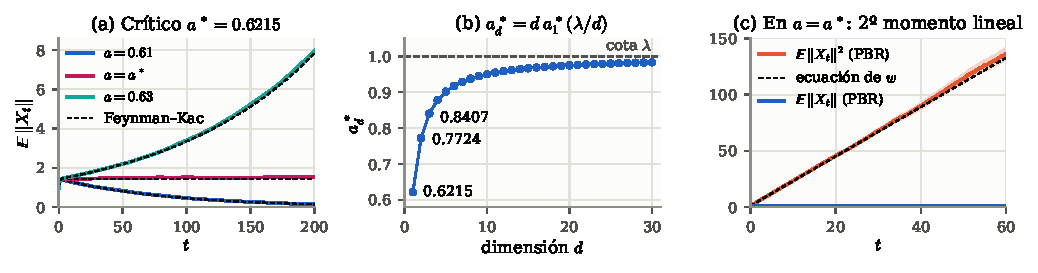
\includegraphics[width=\textwidth]{fig_resumen.pdf}
\captionof{figure}{\small (a) Promedio de partículas vivas con $p(x)=x^2$ y $\lambda=h=1$: simulación del sistema (color) y Feynman--Kac (punteado). (b) Parámetro crítico según la dimensión. (c) En $a=a^*$ la media se estabiliza, pero el segundo momento crece linealmente.}
\label{fig:resumen}
\par}
\vskip 0.2in
]

%\printAffiliationsAndNotice{}

\section{Introducción}
Un paseo aleatorio con ramificación (PBR) es un sistema de partículas en la grilla $x_0+h\mathbb{Z}$ en que cada partícula, de forma independiente, salta a $x\pm h$ a tasa $\lambda$ y se ramifica a tasa $a+p(x)$: tiene dos hijos con probabilidad $p_2=a/(a+p(x))$ o muere con probabilidad $p_0=p(x)/(a+p(x))$. Es decir, nace a tasa constante $a>0$ y muere a tasa $p(x)\geq 0$, que depende de la posición. Se estudia el promedio de la población, $m(t,x)=\mathbb{E}_{\delta_x}\|X_t\|$: cómo calcularlo y cuándo se extingue, crece o se estabiliza. El caso base es $p(x)=x^2$, $\lambda=h=1$.

\section{Desarrollo}
El promedio se calcula de tres maneras. La primera es simular el sistema completo (Monte Carlo), que es costoso. La segunda es la fórmula \textit{Many-to-One}, que usa un solo paseo simple $Z$ de tasa $\lambda$ con un peso:
\begin{equation}
    m(t,x) = \mathbb{E}_x\Big[\exp\Big(\int_0^t \big(a - p(Z_s)\big)\,ds\Big)\Big].
    \label{eq:manytoone}
\end{equation}
La tercera es la ecuación de Feynman--Kac, que es determinista:
\begin{equation}
    \partial_{t} m = L m + (a-p)\,m, \qquad m(0,\cdot)=1,
    \label{eq:feynmankac}
\end{equation}
donde $L$ es el generador del paseo. De \eqref{eq:feynmankac} sale el parámetro crítico $a^*=-\sup\operatorname{spec}(L-p)$: el promedio se comporta como $e^{(a-a^*)t}$ y en $a=a^*$ se estabiliza. Para $p(x)=x^2$ se obtiene $a^*=0.6215$ (Figura~\ref{fig:resumen}a).

A tiempos largos el estimador de \eqref{eq:manytoone} falla: la esperanza la sostienen unas pocas trayectorias que se quedan cerca del origen, con peso de hasta $e^{at}$. Se corrige con la transformada $h$ de Doob.

\section{Resultados}
\textbf{Distintas $p(x)$.} \eqref{eq:manytoone} y \eqref{eq:feynmankac} valen para toda $p\geq 0$, sin pedirle regularidad. El crítico estabiliza el promedio cuando $p$ es confinante ($|x|$, $x^4$), tiene un pozo ($x^2/(1+x^2)$, con $a^*=0.4227$) o es periódica. Si $p\to 0$ en alguna dirección, como en $1/(1+x^2)$ y $(x^+)^2$, resulta $a^*=0$ y no hay crítico positivo. Además $a^*$ depende de la subred de partida: $0.6215$ en $\mathbb{Z}$ y $0.6523$ en $\mathbb{Z}+\tfrac12$.

\textbf{Tasa de salto $\lambda(t)$.} \textit{Many-to-One} sigue valiendo si $\lambda\in L^1_{\mathrm{loc}}$. Feynman--Kac pasa a ser un problema con condición final: para un horizonte $T$, $u(s,x)=\mathbb{E}[\|X_T\|\mid X_s=\delta_x]$ cumple
\begin{equation}
    -\partial_{s} u = \lambda(s)\,L_1 u + (a - x^2)\,u, \qquad u(T,\cdot) = 1,
    \label{eq:backward}
\end{equation}
con $L_1$ el generador de tasa 1, y $m(T,x)=u(0,x)$. Reemplazar $\lambda$ por $\lambda(t)$ en \eqref{eq:feynmankac} da un resultado incorrecto. Los tres métodos coinciden hasta $T=50$. Existe un $a^*$ constante si $\lambda$ converge o es periódica.

\textbf{Grilla en $\mathbb{Z}^d$.} Con $p(x)=\|x\|^2$ y saltos a los $2d$ vecinos con probabilidad $1/2d$, las coordenadas son paseos independientes de tasa $\lambda/d$, de donde $a^*_d=d\,a^*_1(\lambda/d)$: $0.6215$, $0.7724$, $0.8407,\dots$, creciente hacia $\lambda$ (Figura~\ref{fig:resumen}b). Los tres métodos coinciden en $d=2$ y $d=3$.

\textbf{Varianza.} El segundo momento $w=\mathbb{E}_{\delta_x}\|X_t\|^2$ cumple Feynman--Kac con una fuente: $\partial_t w = Lw+(a-x^2)\,w+2a\,m^2$, $w(0,\cdot)=1$. Su umbral es el mismo $a^*$, pero en $a=a^*$ crece linealmente (Figura~\ref{fig:resumen}c): ningún $a$ estabiliza la varianza.

\end{document}
